\documentclass[titlepage,a4paper,11pt]{article}
\usepackage[pdfborder={0 0 0}]{hyperref}
\usepackage{fontspec}
\usepackage[hmargin=2.54cm,vmargin=1.91cm]{geometry}
\usepackage{parskip}
\usepackage{wrapfig}
% TableMagic+shading
\usepackage{multirow}
\usepackage[english]{babel}
\usepackage{longtable}
\usepackage{float}
\usepackage{graphicx}
\usepackage[table]{xcolor}
\usepackage{biblatex}
\usepackage{fancyhdr}
\usepackage{titlesec}
%	-- Some important declarations --
%	-- Section Header: NOTE! It renews the command 

\renewcommand{\baselinestretch}{1.3}
\definecolor{my_color}{HTML}{808080} 
\titleformat{\section}[hang]{\sffamily\bfseries}
{\color{my_color}\Huge\thesection}{0pt}{\linebreak\huge\raggedleft}[{\titlerule[0.5pt]}]

%	-- Bibliography
\bibliography{myrefs}

%	-- Tableshade color
\definecolor{tableShade}{HTML}{F1F5FA}

%	-- Project info
\def \project {Defense of the Guardian Gnome}
\def \objective {guardian gnome}

%	-- Font Style (uses Xelatex engine (Unicode))
%\setromanfont{Century Gothic}

%	-- Date of last run (frontpage)
\date{\today}

\begin{document}
\title{Implementation Description Document\\
 		TDT4240 - XNA Game Project}

\author{Dag Øyvind Tornes\\
 		Sibte-Haider Syed\\ 
		Robin Kåveland Hansen\\}
\maketitle
\newpage
\thispagestyle{empty}
\mbox{}

% Roman numbering until end of TOC
\pagenumbering{roman}
	
% A trick to insert a empty page
\newpage
\thispagestyle{empty}
\mbox{}
% End of trick

% We dont want numbering on the TOC
\pagestyle{empty}
\tableofcontents
\clearpage

% And now we want the normal arabic numbering!
\pagestyle{fancy}
\rhead{\color{my_color}\Huge\thesection}
\lhead{}
\renewcommand{\headrulewidth}{0pt}
\pagenumbering{arabic}

%
% Here we can include all the real "writing"
%
%	\include{file} to get the firstpage for each section nice and neat <3

\pagestyle{empty}

\section{Introduction}
\emph{"This section will describe the purpose of this document, and what it consists of"}
\newpage
	This document describes the requirements that have been developed for \project,
a game developed for the XNA platform. It describes the functional requirements
and thus a high-level overview of how the game should play. There are also some
scenarios for content development that describe the quality requirements imposed
on the system. Chapter \ref{concepts} describes the concept behind the game on
a high level, as well as some discussion around some game design choices that
have been made at this time or will have to be made in the future. Chapter
\ref{funcreq} lays down the functional requirements that were decided on.
Chapter \ref{qualreq} deals with the quality requirements in detail, as well as
some scenarios that might be relevant for \project. Chapter \ref{constraints}
describes in some detail the constraints that were imposed on the game by either
the developers, or the technology used.


\section{Implementation Details}
\emph{"This section will describe a more detailed view of the various parts of the architecture and design"}
\newpage
	
In this section we will describe how the architecture was implemented, and
review how the decisions made during planning turned out.

Some changes were made to accommodate new ideas, and when we found the
architecture lacking. Most of these changes were small however, and we feel
the architecture we designed was a very good fit for what we wished to
accomplish, and solved most of the goals we had set for ourselves.

The list below shows which features we wish to highlight, and were crucial
in implementing the architecture as we had planned it.

\begin{itemize}
	\item \textbf{prograrkSpill.Game} \\
	      Entrypoint for application required by XNA
	\item \textbf{progarkSpillContent} \\
	      Project containing all data
  	\item \textbf{progarkSpill.GameObjects} \\
  	      A modular system for composing game related features
  	\item \textbf{progarkSpill.GameStateStack} \\
  	      Controls the states a game can be in		
	\item \textbf{progarkSpill.GameState : IGameState} \\
	      Controls that decide how application acts in different states 
	\item \textbf{progarkSpill.MenuState : IGameState} \\
	      Controls that decide how application acts in different states 
	\item \textbf{progargspill.Controller} \\
	      Xbox360 gamepad Layer
	\item \textbf{progarkSpill.Renderer} \\
	      View functionality - renders GameState to screen 
	\item \textbf{progarkSpill.Viewport} \\
	      View functionality - renders GameState to screen
\end{itemize}

\subsection{progarkSpill.Game}
This class is added by XNA to any project, and abstracts away many details
about the underlying architecture, and provides hooks for common functions.
It is optional to use, all the features used by this class are provided at
a lower level in XNA if you need more control over how your game runs. We
found it to be adequate for our needs, and have decided to keep it.

In our project we use it for three high-level features. In the LoadContent()
method we create our resource-management system, and initialize our rendering
subsystem.  In the Update() method, we record time spent on the last frame, and
use this to update the game in a time-independent manner. Finally, in the
Render() method, we set the state needed by the rendering-system, and then
allow it to render the current state.

\subsection{progarkSpillContent}
This is a Visual Studio project created by XNA.  It is connected to the
content-management system XNA provides, and allows you to add resources and set
properties on these.

XNA allows you to add quite a few kinds of resources, such as graphics, sound, 
XML and more. We use three of these features, Graphics, Fonts and XML. One
drawback of this method of adding content is that you need to rebuild the
project whenever you add content. XNA does this to allow compression and 
bundling data which can then be sent to the XBOX. This does however free us
from interacting with the XBOX' file system, and we feel it is a fair tradeoff.

\subsection{progarkSpill.GameObjects}
The GameObjects package implements what we have called the \emph{Component-
Based System} in our architecture. It is a very flexible system, which allows
us to reuse much of the games' functionality in different places, allows us
to compose new features with minimum code changes and is an integral part of
our data-driven approach to coding.

Understanding this package is best done by looking at the \emph{Entity} class,
but we will highlight some possibilities the system opens for us.

In short, everything you see on the screen, and quite a few things you don't
see, are implemented as Entities. Each entity is a container for different
components, which have clearly defined responsibilities. There are for 
instance:
\begin{itemize}
    \item Renderables (Used for showing things on screen)
    \item Behviours (Mostly used for AI, but also player control)
    \item Abilities (Which allow entities to interact with the game world)
    \item And many more, see the code for complete coverage.
\end{itemize}

This system allows us extreme flexibility in composing new features, and 
defining the world of our game. The primary guideline when developing this
system was modifiability, but there were some tradeoffs which had to be made.
The system is complex, and takes some time to understand. Complex code hinders
maintainability, which is closely related to modifiability. The endless 
possibilities of this system however far outweigh the downsides.

To show just how flexible this system is, we will go through how two integral
features from the game were implemented using this system. They are the players
avatar in the game, and the entity which allows us to add hostiles to the 
world.

First the player. The important thing to note here is that the player is no
different from a hostile in the game. Sure they have more health and better
weapons (which are defined in data), but they follow the same rules as 
everybody. We do this by creating a custom behaviour for players which read the
state of the XBOX controller. This then directs the players entity, which
updates just as if it were any other creep.

The other example we wish to highlight is creep-spawners. These are responsible
for adding hostiles to the world. They are defined in data, and are invisible
to players (They could however be made visible, for instance creeps might be
deployed from a carrier). In terms of functionality they are as far removed 
from players as one could possibly come, but are still implemented using the
same base classes.  A creep-spawner is an entity whose only ability is to spawn
hostiles. The quite literally shoot hostiles into the world (using the exact
same code that players use to shoot their main cannon)

\subsection{progarkspill.GameStateStack}
A game usually has different phases, such as showing a splash-screen, menus and
obviously playing the game itself. We wanted these features, and asked 
ourselves how we could do this as elegantly as possible.  Our first solution
was to implement an event-system which would queue state-changes and change
states transparently to the states. We decided early on however that we were
over-engineering the problem, and changed this to a simple stack of states.

Each state has access to this stack, and can add or remove new states. We then
call methods on the top element of the stack, and everything works out neatly.
This solution introduces some coupling in the code, for instance any state 
which can lead into another state must know of the other state. An example is
the main menu which must know of the in-game state in order to start the game.
This would be avoided by using the aforementioned event-system, but we feel
our current system works well enough, and the downsides are small compared to
the extreme simplicity of this system.

\subsection{progarkSpill.GameState}
This class represents the state of being in the playable portion of the game. 
It is a good place to start understanding the sequence of logic in the game.

The class is unfortunately very large, and has many responsibilities. For 
instance this is where we store the current level, it contains a list of all
players and hostiles, and also encodes the winning and losing conditions. It is
the closest we have come to a \emph{god-object}, so-named because it knows
everything and can do anything, which plagues many game architectures.

This is the one thing in our project which we are truly unhappy with, and the
first thing to be revised if we had more time to do it. There is not a single
redeeming feature to having a large monolithic class with such disparate
responsibilities, aside from the fact that it is incredibly easy and a quick
solution.

\subsection{progarkSpill.MenuState}
This is a group of classes which represents the different menus in the game.
While they are simple and powerful, we do wish we could make these more data-
driven, and perhaps a lot more pretty.

Each class has two methods which implements most of the functionality of that
menu. A total of four menus were implemented, the main menu, two menus 
displayed  after winning or losing the game, and a pause-menu.

\subsection{progarkSpill.Controller}
This is a single class containing nothing but static methods and members. It
was created as a layer of abstraction above XNAs similar GamePad class, but
contains one more features we needed for our game, namely tracking the time a
certain button was pressed. It would also be the place any other controller-
related features were added. This class resembles the \emph{Singleton-pattern}
closely, in that it provides global access and a single point of responsibility
for controllers. It is not implemented in the way that singletons usually are
however. We chose to use all static members, and drop the silly getInstance()-
interface one often sees in this pattern.

\subsection{progarkSpill.Renderer}
This subsystem is the only way to display graphics on the screen, and an
instance to it is passed around to nearly all portions of the code. It was
designed to be extendable and configurable in most ways, but we never needed
this extensibility. The renderer could, if needed, maintain internal lists of
all submitted render-jobs, reorder them for optimization, or share state 
between jobs for extensibility. We also planned to use Post-Processing effects,
but this feature was scrapped due to time-constraints.

What we wound up with is a class which can display graphics in many ways, and
which can be configured by the game through the IRenderable interface. Due to
some miscommunication in the start of the project the interface was not 
implemented as planned, but all the features we planned for (with the noted
exception of the effects) are still available.

\subsection{progarkSpill.ViewPort}
This is a class which handles transforms between the game's coordinate-system
and the screen. It was implemented to allow different screen-sizes (i.e. on
HD-Ready and Full-HD screens), and to allow us to think in terms of a natural
unit of measurement such as meters, instead of thinking in terms of pixels.
	
\section{User manual}
\emph{"This section will describe how you can run the game"}
\newpage
	There are two ways two play the game, either by deploying the game to the Xbox 360 and play it on the console, or 
run the game on Windows with two Xbox 360 controllers attached. We have written a manual for both, so the reader can 
test the game according to his/her preferences. 

\subsection{Xbox 360}

In order to play the game on the Xbox 360 Console, there are several prerequisites to take into account. Firstly, 
the following is mandatory\cite{deploy}:

\begin{itemize}
	\item Computer running Windows with XNA Game Studio 4.0 
	\item Xbox 360 Console with two controllers
	\item XNA Game Studio Connect on the Xbox 360 Console 
	%\item Atleast an Silver Xbox LIVE membership \\
	%\item XNA Creators Club premium membership \\
	\item Hard drive on the Xbox 360 to deploy the game onto 
\end{itemize}

\subsubsection{Connecting the Xbox 360 Console with XNA Game Studio 4.0}

Note! In order to download \textbf{XNA Game Studio Connect}, the Xbox 360 console needs an internet connection. \\

\begin{enumerate}
	\item On the Xbox 360 Console, navigate to \textbf{Game Marketplace}.
	\item Select \textbf{Explore Game Content} and then \textbf{Browse}. 
	\item When your at the \textbf{All Games} screen browse to \textbf{Genre} and select \textbf{Other}. 
	\item Scroll to \textbf{XNA Creators Club} and select it. 
	\item From this pane, select \textbf{All Downloads}, then select \textbf{XNA Game Studio Connect}. 
	\item \textbf{Confirm Download} to begin downloading. 
\end{enumerate}

In order to deploy the game to the Xbox 360 console, the development computer and the Xbox 360 needs to be on the same subnet on the local network. If the computer and console is behind the same router, it is very likely that you're on the same subnet. In order to deploy the game a \textbf{connection key} needs to be generated. \\

\begin{enumerate}
	\item On the Xbox 360 Console, go to \textbf{My Xbox} and select \textbf{Game Library}. 
	\item then go to \textbf{Collections} tab and select \textbf{Community Games}. 
	\item Select \textbf{XNA Game Studio Connect} and then select \textbf{Launch}. 
	\item The XNA Game Studio connect screen will appear: \\ \begin{center}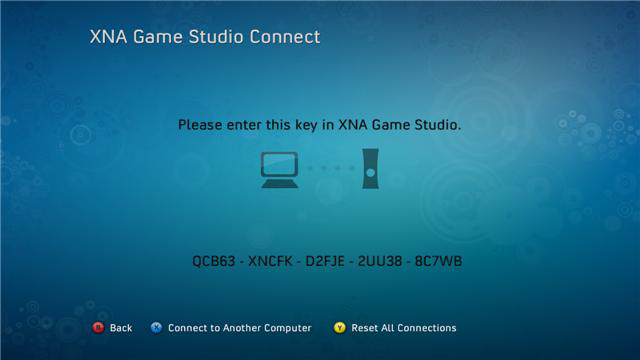
\includegraphics[scale=0.5]{graphics/connect}\end{center}
	\item If a \textbf{Connection Key} is displayed go to step \ref{generated}. 
	\item If the \textbf{Connection Key} does not appear, the Xbox 360 console could already be connected to this computer. The game studio supports multiple connection keys for multiple computers. To add a new connection press \textbf{X}. 
	\item \label{generated} On your computer, go to the \textbf{Start} menu, select \textbf{programs} and then select \textbf{XNA Game Studio 4.0}. 
	\item Launch the \textbf{XNA Game Studio Device Center}.
	\item Click \textbf{Add Device} \\ \begin{center}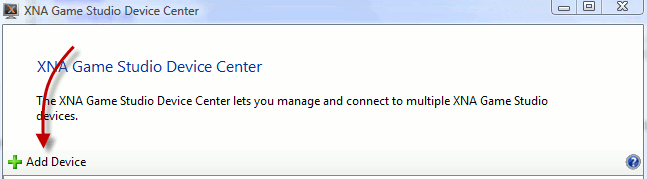
\includegraphics[scale=0.75]{graphics/add_device}\end{center} 
	\item Select the type type of device to be \textbf{Xbox 360} \\ \begin{center}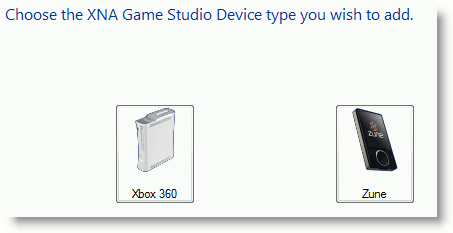
\includegraphics[scale=0.75]{graphics/type_of_device}\end{center} 
	\item Enter a name for the console and press \textbf{Next}. 
	\item Enter the connection key that is displayed in the XNA Game Studio Connect on the Xbox 360 console. 
	\item Once you have typed in the correct key, press \textbf{Next} on the \textbf{XNA Game Studio Devices} dialog box. 
	\item The XNA Game Studio Device center will test the connection. If it fails, pay attention to the error message of the dialog box. If it did not result from a mismatched key, please refer to \cite{troubleshoot}. 
	\item Click \textbf{Finish}. The console will now be listed in the XNA Game Studio Device Center  
\end{enumerate}

\subsubsection{Deploying the game to Xbox360}

\begin{enumerate}	
	\item On the development computer, fire up the project in Visual Studio.
	\item Then go to the Xbox 360 console and go to \textbf{My Xbox} and then select \textbf{Game Library}. 
	\item From \textbf{Game Library}, go to the \textbf{Collections} tab and then select \textbf{Community Games}
	\item Select \textbf{XNA Game Studio Connect} and then select Launch, which will display a screen like this: \\ \begin{center}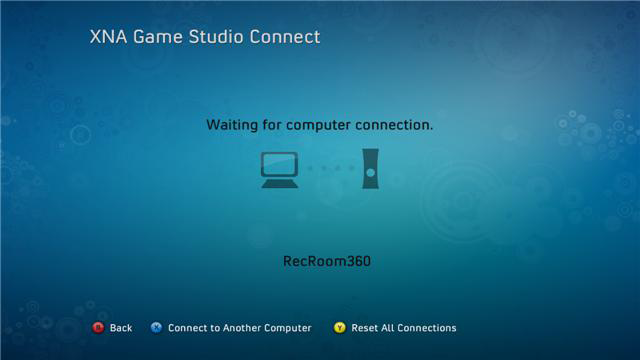
\includegraphics[scale=0.5]{graphics/connect2}\end{center}
	\item On your computer, build the project, deploy the needed files Xbox 360 and then run.
	\item Now you have deployed the game. 
	\item The game will appear in \textbf{Recent games} in the \textbf{Game Library}.	 
\end{enumerate}

\subsection{Playing the game on a (Windows) computer}

In order to play the game on a Windows computer, you need at least two Xbox 360 controllers. To connect a controller to the PC, you will need a USB cable connector from the controller to the computer. From this point, simply execute the executable file, and play! 




\section{Test - Plan and Reporting}
\emph{"This section contains the test reports for both the functional and quality requirements"}
\newpage
	Before evaluating each functional requirement and quality requirement, table \ref{tab:implemented_reqs} lists what requirements that we as developers have implemented. That does not imply that every requirement is working, but rather what has been implemented and needs testing. 

The requirements that haven't been implemented, will not be tested. We refer to the \emph{requirements description document} for more in depth information on the requirements

\begin{table}[H]
	%\resizebox{\textwidth}{!}{
	\begin{center}
	\rowcolors{0}{white}{tableShade}
	\begin{tabular}{p{2cm} | p{2cm} | p{4cm}}
    	\hline
		\textbf{ID} 			& 	\textbf{Priority}	&	\textbf{Implemented}\\ 
		\hline
		FR1			&	High				&	Yes						\\
		FR2			& 	High				& 	Yes						\\
		FR3			& 	High 				& 	Yes						\\
		FR4			&	High				& 	Yes 					\\
		FR5			& 	High				& 	Yes						\\
		FR6			& 	High				& 	Yes						\\
		FR7			& 	High				& 	Yes						\\
		FR8			&	High				&	Yes						\\
		FR9			&	High				& 	Yes						\\
		FR10		&	High				& 	\textbf{No} 			\\
		FR11		&	High				&	Yes\*					\\
		FR12		&	High				&	Yes						\\
		FR13		&	Medium				&	Yes						\\
		FR14		&	Medium				& 	Yes						\\
		FR15		&	Medium				& 	Yes						\\
		FR16		&	Low					&	\textbf{No}				\\
		FR17		&	High				&	Yes						\\
		FR18		&	Medium				& 	\textbf{No}				\\
		FR19		&	Medium				&	Yes						\\
		FR20		&	Medium				&	Yes						\\
		FR21		&	High				&	Yes						\\
		\hline
    \end{tabular}
\end{center}
	\caption{Implemented functional requirements}
	\label{tab:implemented_reqs}
\end{table}


	
\section{Relationship with the architecture}
\emph{"This section lists the inconsistencies between our architecture and the implementation. We will present, reason and discuss them."}
\newpage	
TODO: Add / list inconsistencies beetween the architecture and implementation, give reason and discuss if they should
	have been discovered earlier by e.g. ATAM. (BLAME THE OTHERS!!!;)
	Add the func reqs here?
	\subsection{Functional Requirements that were not implemented}

Blabla DISCUSSIOn

\begin{table}[H]
	\resizebox{\textwidth}{!}{
	\rowcolors{0}{white}{tableShade}
	\begin{tabular}{p{5cm} | p{12cm}}
    	\hline
		\textbf{ID:} 			& 	\textbf{FR10} 												\\ 
		\hline
    	
		\textbf{Priority:}		&	High														\\
		\textbf{Description}	& 	A hero / player has a limited amount of resources\\ 
		\textbf{Rationale}		& 	The game is cooperative, and adding depth to the game		\\
		\hline
		\textbf{Exclusion rationale} & Time, architecture supports adding this feature easily. \\
    \end{tabular}
	\label{tab:functional10}}
\end{table}


\begin{table}[H]
	\resizebox{\textwidth}{!}{
	\rowcolors{0}{white}{tableShade}
	\begin{tabular}{p{5cm} | p{12cm}}
    	\hline
		\textbf{ID:} 			& 	\textbf{FR16} 												\\ 
		\hline
    	
		\textbf{Priority:}		&	Low															\\
		\textbf{Description}	& 	A hero can buy items to enhance abilities or skills			\\ 
		\textbf{Rationale}		& 	The game is cooperative										\\
		\hline
		\textbf{Exclusion rationale} & Relies heavily on resources. So removed due to FR10 \\
    \end{tabular}
	\label{tab:functional16}}
\end{table}

\begin{table}[H]
	\resizebox{\textwidth}{!}{
	\rowcolors{0}{white}{tableShade}
	\begin{tabular}{p{5cm} | p{12cm}}
    	\hline
		\textbf{ID:} 			& 	\textbf{FR18} 													\\ 
		\hline
    	
		\textbf{Priority:}		&	Medium															\\
		\textbf{Description}	& 	Passive abilities does not need to be activated by the player	\\ 
		\textbf{Rationale}		& 	According to the conceptual model of this genre of games		\\
		\hline
	\textbf{Exclusion rationale} & 	We have only added active abilities. \\
 	\end{tabular}
	\label{tab:functional18}}
\end{table}

\begin{table}[H]
	\resizebox{\textwidth}{!}{
	\rowcolors{0}{white}{tableShade}
	\begin{tabular}{p{5cm} | p{12cm}}
    	\hline
		\textbf{ID:} 			& 	\textbf{FR21} 													\\ 
		\hline
    	
		\textbf{Priority:}		&	High															\\
		\textbf{Description}	& 	Each player will have his score shown while playing: kills + points \\ 
		\textbf{Rationale}		& 	To introduce a competitive scenario even though it is cooperative	\\
		\hline
		\textbf{Exclusion rationale} & NOT added ETA???? \\
    \end{tabular}
	\label{tab:functional21}}
\end{table}



\section{Problems, Issues and Points Learned}
\emph{"This section will list problems and issues with this document, or the implementation process. We will also discuss the project as a whole"}
\newpage
	The project team only consisted of three members which severely impacted how much the team could manage to implement. During the implementation we learned that two more members were to join our team, but that did not seem to be true. We never heard from those members. We are very proud that we managed to produce so much as we did, given the size of the group.  

Illness was a problem for the project team. Absence of one member made a huge impact on the team. Luckily we did not to much of those, but it did make a huge impact every time. Due to all this, we have been forced to prioritize. We have focused more on the actual implementation, than revising the initial \emph{Architectural Description Document} and \emph{Requirements Description Document}. We have tried to focus more on this document and the code, convincing ourselves that we have learned from the feedback from the staff, even though we haven't addressed them all e.g. like COTS etc.   

The changes we did occurred have been mentioned in this document. 


 

	
%\pagestyle{empty}
\section{Revision history}

%\pagestyle{fancy}
TODO: FILL ME UP, WHAT; WHERE; WHEN; WHY!

\begin{table}[H]
  \begin{tabular}{| c | c | c |}
    \hline
    0.1 & 01.03.2011 & Initial revision of this document. \\
    \hline
  \end{tabular}
\end{table}
\end{document}
